\documentclass[9 pt]{article}
\usepackage{amsmath, amssymb, color, xcolor, amsthm}
\usepackage{graphicx, wrapfig, float, caption, dsfont, bbm}
\usepackage{fullpage}
\usepackage[backref=page, hidelinks, colorlinks=true, citecolor=blue!60!black!100]{hyperref}
\usepackage{tikz}
\usetikzlibrary{arrows.meta, shapes}
\usepackage{caption, subcaption}
\usepackage[super]{natbib} % gives us \citet: Author (year) and \citep: (Author; year)
\usepackage{authblk}

\usepackage{multicol}

\newcommand{\plr}[1]{{\color{blue}\it #1}}
\newcommand{\jss}[1]{{\color{olive}\it #1}}
% \newcommand{\ddt}{\frac{d}{dt}}
\newcommand{\ddt}{\dot}
\newcommand{\ro}{{ro}}
\newcommand{\nro}{{\bar{r}o}}
\newcommand{\rno}{{r\bar{o}}}
\newcommand{\nrno}{{\bar{r}\bar{o}}}
\newcommand{\reachable}{\mathcal{R}}
\newcommand{\unobservable}{\bar{\mathcal{O}}}
\newcommand{\R}{\mathbb{R}}
\newcommand{\E}{\mathbb{E}}
\renewcommand{\P}{\mathbb{P}}
\newcommand{\pda}{\frac{\partial}{\partial A_{ij}}}
\newcommand{\ind}{\mathds{1}}

\newcommand{\A}{\mathcal{A}}
\newcommand{\diag}{\text{diag}}
\newcommand{\1}{\mathbbm{1}}

\DeclareMathOperator{\spn}{span}

\newtheorem{theorem}{Theorem}
\newtheorem{lemma}{Lemma}
\newtheorem{definition}{Definition}
\newtheorem{example}{Example}

\begin{document}

\section*{The evolution of phenotypically invariant gene networks with implications for speciation, adaptation, and neutral variation}
{\centering
Joshua S. Schiffman$^{\dagger}$ \qquad Peter L. Ralph$^{\dagger \ddagger}$ \\
$^{\dagger}$University of Southern California, Los Angeles, California \qquad $^{\ddagger}$University of Oregon, Eugene, Oregon \\
\texttt{jsschiff@usc.edu} \qquad \texttt{plr@uoregon.edu}
\\
}

\begin{multicols}{2}


\section*{Abstract}
  \textbf{
I will outline an analytical theory to study the evolution of biological systems such as gene regulatory networks, borrowing insight and tools from control engineering, systems identification, and dynamical systems theory. I will describe a null model of regulatory network evolution by analytically describing the set of all linear gene networks (of any size) that produce identical phenotypes -- and the evolutionary paths connecting them. In the idealized case of a perfectly adapted population, constant selection, and a static environment, we observe neutral evolution as a random walk over the phenotypically- invariant network-space. Under neutral conditions, this model can provide descriptions of expected network size and connectivity under mutation-selection equilibrium, estimate the rate of regulatory rewiring, and the rates at which Dobzhansky-Muller incompatibilities arise in reproductively isolated populations. This analysis provides insight into the mechanisms and parameters important for understanding developmental systems drift, network rewiring, evolvability, epistasis, and speciation, as well as the tenuous connection between network architecture and function. 
}
\section*{Introduction}

Bridging the gulf between an organism's genome and phenotype is a poorly understood and complex molecular machinery. Progress in a suite of biological subdisciplines is stalled by our general lack of understanding of this molecular machinery: with respect to both its function and evolution. There does exist a growing body of experiment and data on the evolutionary histories and molecular characterizations of particular gene regulatory networks \citep{jaeger2011gap, davidson2006gene, israel2016comparative}, as well as thoughtful verbal and conceptual models \citep{true2001developmental, gwagner1, weiss2000phenogenetic, edelman2001degeneracy}. However, as Hardy and Weinberg taught us over a century ago, verbal theories are often insufficient, if not downright misleading \citep{hardy1908mendelian, weinberg1908vererbungsgesetze, servedio2014not}. This is especially pertinent given the staggering complexity and scope of contemporary research programs. This outlook necessitates the advancement of conceptual frameworks of such precision, only mathematics will suffice. Previously it has been suggested that any idealized study of evolution is incomplete without a mathematically sufficient description of the genotype, phenotype, and transformation from one to the other \citep{Lewontin1974genetic}.%Here we outline an analytical theory to study the evolution of biological systems, borrowing insight and methods from control engineering, systems identification, and dynamical systems theory. 

%Presently, we focus on the neutral evolution of genetic regulatory networks. That is, we analytically describe the set of all linear gene networks (of any size) that produce identical phenotypes -- and the evolutionary paths connecting them. In the idealized case of a perfectly adapted population, constant selection, and a static environment, we observe evolution under the ``conservation of phenotype'' as a Brownian motion over phenotypically-invariant network-space. This analysis provides insight to the mechanisms and parameters important for understanding developmental systems drift, network rewiring, evolvability, epistasis, and speciation, as well as the tenuous connection between network architecture and function.


%It is commonly taught that an organism's genome contains the heritable material 
%that natural selection filters and that an organism's phenotype directly determines its
%evolutionary fitness. Between genotype and phenotype is an often complicated and poorly
%undrstood molecular machinery -- and it is a major goal common to many different disciplines
%within the life sciences to elucidate its form, function, and evolution. These aims are
%delicately intertwined and a comphrehensive understanding of a system's evolution requires
%an understanding of its function and vice versa.

The molecular machinery, interacting with the environment, and bridging genotype to phenotype
can be mathematically described as a dynamical system -- or a system of differential equations\citep{jaeger2015comet}.
 Movement in this direction is ongoing, as researchers have begun to study 
the evolution of both abstract \citep{wagner1994evolution, wagner1996does,  siegal2002waddington, bergman2003evolutionary} and empirically inspired computational and mathematical models of gene regulatory networks (GRNs) \citep{mjolsness1991connectionist, jaeger2004dynamic, maria1, vitaly1, vitaly2, crombach2016gap, wotton2015quantitative, chertkova2017insilico}. If we allow the reasonable assumption that the genotype-phenotype map can be represented as a system of differential equations, we can immediately discuss its evolution and function in a much more mechanistic, yet general, manner. 

In some fields that seek to fit parametric models to experimental data, such as control
theory, chemical engineering, and statistics, it is well known that mathematical models
can fundamentally be \emph{unidentifiable} and/or \emph{indistinguishable} -- meaning that 
there can be uncertaintity about an inferred model's parameters or even its claims about
causal structure, even with access to complete and perfect data \citep{bellman1970structural, grewal1976identifiability, walter1984structural}. Models with different 
parameter schemes, or even different mechanics can be equally accurate, but still not
\emph{actually} agree with what is being modelled. In control theory, where electrical 
circuits and mechanical systems are often the focus, it is understood that there can be an 
infinite number of ``realizations,'' or ways to reverse engineer the dynamics of a black box,
even if all possible input and output experiments on the black box are performed \citep{kalman1963mathematical, anderson1966equivalence, zadeh1976linear}. In chemical
engineering, those who study chemical reaction networks sometimes refer to the fundamental
unidentifiability of these networks as ``the fundamental dogma of chemical kinetics'' \citep{craciun2008identifiability}. In computer science, this is framed as the relationship among processes that simulate one another \citep{van2004equivalence}.
Although this may frusturate the occasional engineer or scientist, viewed from another angle,
the concepts of unidentifiability and indistinguishability can provide a starting point for
thinking about externally equivalent systems -- systems that evolution can explore, so long
as the parameters and structures can be realized biologically. In fact, evolutionary
biologists who study homology and analogy are very familiar with such functional symmetries; macroscopically identical phenotypes in even very closely related species can in fact be divergent at the molecular and sequence level \citep{true2001developmental, tsong2006evolution, hare2008sepsid, vierstra2014mouse, stergachis2014conservation, taylor2016diverse, matsui2015regulatory}.

In this paper we propose a framework to study the evolution of biological systems. To begin, we focus on the evolution of an idealized population. We consider the evolution of a perfectly adapted, large population, evolving in a static environment for an infinite number of generations. Under these ideal circumstances, we expect to observe a ``conservation of phenotype,'' where the population explores the manifold of phenotypically-invariant (or symmetric) genetic and developmental architecutres. We would like to understand which parameters influence the distribution of a population along the manifold of phenotypically invariant genetic systems. Further, we can show how dispersion along this manifold contributes to speciation and evolvability. 

\section*{The Model I: Gene Networks as Linear Systems}

  Organisms' phenotypes are constructred by gene by gene by environment interactions. Here we simply define the phenotype to be the organismal temporal molecular dynamics directly under natural selection. The \emph{what}, \emph{when}, and \emph{where}, of an organism's molecules that are physiologically or otherwise relevant for survival. Thus we say that some function $\phi(t)$ is a phenotype where, 
  \begin{align}
    \phi(t) = \int_{0}^{\infty} h(t) u(t) dt  ,
  \end{align}
  and $h(t)$ is the \emph{impulse response} of the system and $u(t)$ is the \emph{input} function, both functions of time $t$. The input can be interpreted as the environment, as initial conditions, or otherwise, depending on the biological specifics under study. 

  Essentially the phenotype $\phi(t)$ is a consequence of an organism's specific gene by gene interactions, given by $h(t)$, reacting further with the local environment, given by $u(t)$. 

  We describe the impulse response as, 
  \begin{align}
    h(t) = C e^{A t} B
  \end{align}
  where $A$ is a gene network -- a square matrix, and $B$ filters and translates the input to the system. The form of $B$ determines precisely how the state of the external environment influences the internal gene network. $C$ filters and translates the dynamics of the system and precesily determines the output, that is, what is visible to selection. 

  Generally $A$ can be any real $n \times n$ matrix, $B$ any $n \times \ell$, and $C$ any $\ell \times n$ dimensional matrix. However, for simplicity in exposition (and without loss of generality) we set $\ell = 1$, so that $B$ and $C$ are simply vectors of length $n$.

  Although $\phi(t)$ describes the phenotype given an input, $h(t)$ describes the phenotype subject only to an impulse -- an input present initially and absent immediately thereafter. Typically, a system $\Sigma$, is defined as,
  \begin{align}
    \Sigma = \left\{ \begin{array}{ll} \dot{\kappa}(t) &= A \kappa(t) + B u(t) \\ \phi(t) &= C \kappa(t) \end{array} \right.
  \end{align}
  Variables have the same identities as described above and $\kappa(t)$ is a vector of molecule concentrations at time $t$. Therefore the molecular concentrations at a specific time are completely determined by the input and gene by gene interactions. Lastly, a portion and/or combination of these molecules, $\phi(t)$, are ``observed'' by selection (this is in constrast to $\kappa(t)$ -- the \emph{kryptotype} -- as it is ``hidden'' from direct selection).

  \begin{example}[Oscillating Gene Network: Circadian Rhythm]
    \begin{align*}
      A = \begin{bmatrix} 0 & 1 \\ -1 & 0 \end{bmatrix} , \qquad B = \begin{bmatrix} 1 \\ 1 \end{bmatrix}, \qquad C = \begin{bmatrix} 1 & 0 \end{bmatrix}
    \end{align*}
    \begin{align*}
      \Sigma = \left \{ \begin{array}{ll} \dot{\kappa}(t) &= \begin{bmatrix} 
        0 & 1 \\ 
       -1 & 0 
        \end{bmatrix} \kappa(t) + \begin{bmatrix} 1 \\ 1 \end{bmatrix} u(t) \\ 
          \phi(t) &= \begin{bmatrix} 1 & 0 \end{bmatrix} \kappa(t) \end{array} \right.
     \end{align*}

      \begin{align*}
        h(t) = \sin(t) + \cos(t)
      \end{align*}

    \begin{figure}[H]
        \begin{center}
            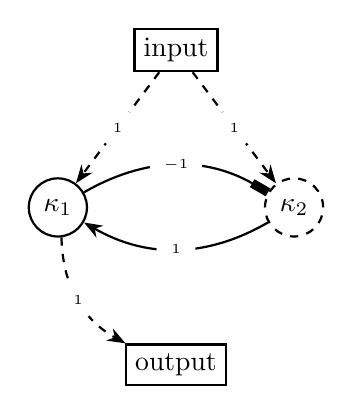
\begin{tikzpicture}
            \begin{scope}[every node/.style={circle,thick,draw}]
                \node (A) at (0,0) {$\kappa_{1}$};
                \node[dashed] (B) at (3,0) {$\kappa_{2}$};
                \node[shape=rectangle] (U) at (1.5,2) {input};
                \node[shape=rectangle] (y) at (1.5,-2) {output};
            \end{scope}

            \begin{scope}[>={Stealth[black]},
                          every node/.style={fill=white,circle},
                          every edge/.style={draw=black, thick}]
                \path [->, >=Rectangle] (A) edge[bend left] node {\tiny $-1$} (B);
                \path [->] (B) edge[bend left] node {\tiny $1$} (A); 
                \path[->] (U) edge[dashed] node {\tiny $1$} (A);
                \path[->] (U) edge[dashed] node {\tiny $1$} (B);
                \path[->] (A) edge[dashed,bend right] node {\tiny $1$} (y);
            \end{scope}
            \begin{scope}[>={Stealth[black]},
                          every edge/.style={draw=black, thick}]
                %\path [->] (A) edge[loop left] node {\tiny $\lambda_{1}$} (A);
                %\path [->] (B) edge[loop left] node {\tiny $\lambda_{2}$} (B);
            \end{scope}

            \end{tikzpicture}
        \end{center}
        \caption{
            Diagram of Example \ref{ex:osc} in the text.
            \plr{explain what arrows mean if nec}
            \label{fig:oscillator_diagram}}
    \end{figure}
    \begin{figure}[H]
      \centering
      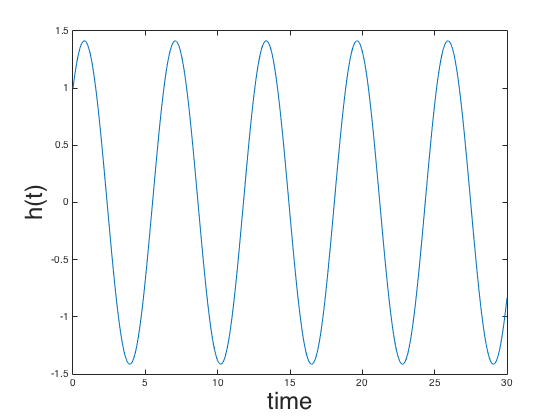
\includegraphics[width=0.5\textwidth]{osc_impulse}
    \end{figure}
  \end{example}

  \section*{The Model II: Linear Evolutionary Systems}

  Systems with identical external dynamics do not necessarily have identical internal dynamics. Any linear and minimal system -- minimal, informally meaning that the system's external dynamics are achieved with the fewest possible number of internal components -- has identical external dynamics up to a change of coordinates. 
  \begin{align}
    h(t) &= C e^{A t} B \\
    &= C V^{-1} e^{V A V^{-1} t} V B \\
    &= C V^{-1} V e^{A t} V^{-1} V B \\
    &= C e^{A t} B
  \end{align}
  Two systems, $\Sigma = \{ A, B, C \}$, and $\bar{\Sigma} = \{\bar{A} = VAV^{-1}, \bar{B} = VB, \bar{C} = CV^{-1} \}$, have the same dynamics if they are related by a change of coordinates. 

  Although systems may not be identifiable beyond a change of coordinates, at present we are primarily interested in a subset of these systems. That is, systems that not only have equivalent external dynamics, but also equivalent input and output relationships. Formally, this means systems related by a change of coordinates (any invertible matrix $V$) that leaves $B$ and $C$ invariant:
  \begin{align}
    VB &= B \implies \bar{B} = B \\
    CV &= C \implies \bar{C} = C
  \end{align}
  In other words systems with varying genetic architectures yet identical selection pressures, environment, and phenotype. 

  Define $V(\tau)$ as the parameterized change of coordinates matrix that preserves $B$ and $C$, with $\tau$ a vector of free parameters. The set of \emph{all} phenotypically invariant (minimal) gene networks is, 
  \begin{align}
    A(\tau) = V(\tau) A(0) V^{-1}(\tau) ,
  \end{align}
  and a \emph{Linear Evolutionary System} is, 
  \begin{align}
    \Sigma(\tau) = \left\{ \begin{array}{ll} \dot{\kappa}(t) &= A(\tau) \kappa(t) + B u(t) \\ \phi(t) &= C \kappa(t) \end{array} \right .
  \end{align}
  \begin{example}[External Equivalence does not imply internal equivalence]
    Gene 1 dynamics (blue) are equivalent for network architectures $A(0)$ and $A(2)$, however the internal dynamics containing gene 2 (orange) are very different.
  \begin{figure}[H]
    \centering
    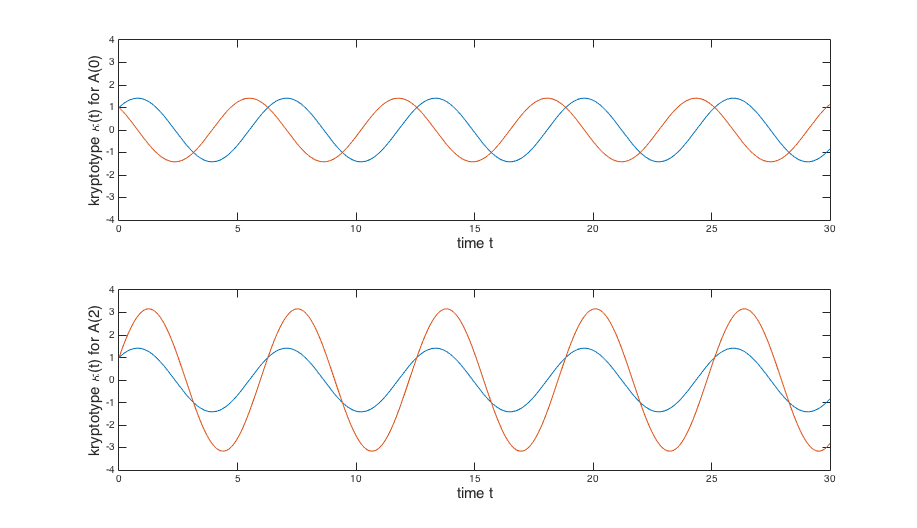
\includegraphics[width=0.5\textwidth]{osc_A0_A2_both_compare}
    %\caption{Gene 1 dynamics (blue) are equivalent for network architectures $A(0)$ and $A(2)$, however the internal dynamics containing gene 2 (orange) are very different.}
  \end{figure}
  \end{example}
  Evolution thus proceeds as a random walk in phenotypically invariant network space. 

  \begin{align}
    A(\tau) \xrightarrow{T} A(\tau + \epsilon)
  \end{align}
  After evolutionary time $T$, the population's gene network architecture evolves from $A(\tau)$ to $A(\tau + \epsilon)$ with a probability inversely proportional to the magnitude of $\epsilon$ and proportional to the magnitude of $T$. 
\jss{Change in $\tau$ is tracking movement of population mean, not ``macro'' evolutionary change, as interpreted previously.}
  \begin{align}
    \Delta_{\tau} &= \left\lVert \frac{d}{d \tau} \text{vec} \left[A\left(\tau\right)\right] \right\rVert^{-1} \\
    A(\tau) &\xrightarrow{\mu} A(\tau \pm \mu \Delta_{\tau})
  \end{align}
  \begin{example}[All Phenotypically Equivalent Oscillators]
    \begin{align*}
      A(\tau) &= \begin{bmatrix} 1 & 0 \\ \tau & 1-\tau \end{bmatrix} \begin{bmatrix} 0 & 1 \\ -1 & 0 \end{bmatrix} \begin{bmatrix} 1 & 0 \\ \frac{\tau}{\tau-1} & \frac{-1}{\tau-1} \end{bmatrix} \\
        B &= \begin{bmatrix} 1 \\ 1 \end{bmatrix}, \qquad C = \begin{bmatrix} 1 & 0 \end{bmatrix} \\
          h(t) &= \sin(t) + \cos(t) \qquad \forall \ \tau \neq 1
    \end{align*}
    \begin{figure}[H]
    \centering
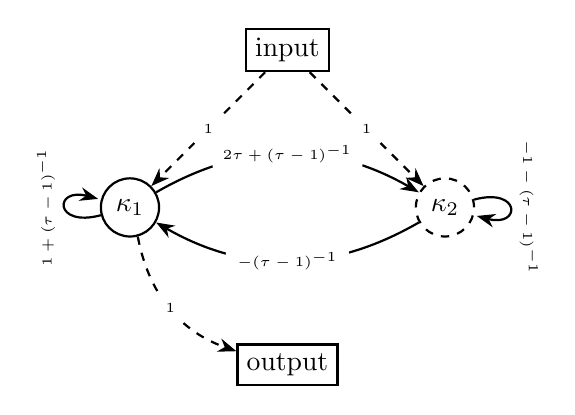
\begin{tikzpicture}
\begin{scope}[every node/.style={circle,thick,draw}]
  \node (A) at (0,0) {$\kappa_{1}$};
    \node[dashed] (B) at (4,0) {$\kappa_{2}$};
    \node[shape=rectangle] (U) at (2,2) {input};
    \node[shape=rectangle] (y) at (2,-2) {output};
\end{scope}

\begin{scope}[>={Stealth[black]},
              every node/.style={fill=white,circle},
              every edge/.style={draw=black, thick}]
    \path [->, sloped] (A) edge[bend left] node {\tiny $2 \tau + (\tau-1)^{-1}$} (B);
    \path [->, sloped] (B) edge[bend left] node {\tiny $-(\tau-1)^{-1}$} (A); 
    \path[->] (U) edge[dashed] node {\tiny $1$} (A);
    \path[->] (U) edge[dashed] node {\tiny $1$} (B);
    \path[->] (A) edge[dashed, bend right] node {\tiny $1$} (y);
\end{scope}
\begin{scope}[>={Stealth[black]},
              every edge/.style={draw=black, thick}]
    \path [->] (A) edge[loop left] node[sloped, anchor=center, above] {\tiny $1 + (\tau-1)^{-1}$} (A);
    \path [->] (B) edge[loop right] node[sloped, anchor=center, above] {\tiny $-1 - (\tau-1)^{-1}$} (B);
\end{scope}

\end{tikzpicture}
    \end{figure}
  \end{example}
  \section*{Phenotypic Invariance}
    First we focus on a simple evolutionary scenario: a large population, perfectly adapted, and in a constant environment. In this circumstance we expect phenotype to be conserved throughout evolutionary time. As such we should only expect the phenotype to change as a consequence of genetic drift (small effective population size), adaptation to new selective and/or environemental pressures. These phenotypic variations should yield distinct signatures. Adaptative changes will change the optimal impulse response function $h(t) \xrightarrow{adaptation} h'(t)$. Genetic drift registers as an increase in the intrapopulation variation in $h(t)$. 
    
    Presently we ask two questions, (1) holding $\phi(t)$, $h(t)$, and $u(t)$ constant for evolutionary time $T$, how much do we expect gene network organization to drift, and (2) does this contribute to speciation, primarily via the fixation of reproductive incompatibilities?

    \begin{example}[Not all minimal gene networks can drift]
      If a gene network is minimal and all the molecular species involved in the network are under selection, such that $C$ is the $n \times n$ identity matrix  ($C = I_{n}$), the only acceptable  change of coordinate matrix is the identify matrix.
     
     \begin{align}
        C \lor B &= I \\
        IV^{-1} &= I \\
        \iff V &= I
      \end{align}
      \end{example}
      \begin{example}[All Non-Minimal Gene Networks can Drift]
      
      Despite the existence of a unique genetic architecture in the minimal case, there still exists an infinite number of systems with larger networks that have identical external dynamics. 
      \begin{align}
        h(t) &= \widehat{h}(t) \iff \\ 
        CA^{\jmath}B &= \widehat{C} \widehat{A}^{\jmath} \widehat{C} \qquad \text{for } \jmath = 0, 1, \dots
      \end{align}
      Any two systems with equivalent impulse responses will have equivalent phenotypes.
      \end{example}

      \plr{add Kalman decomposition stuff here}

      \subsection*{Speciation via Reproductive Incompatibility}

      %Define reproduction in diploids as first, the recombination of unlinked genes to make gametes, and second, as the averaging of two individual parental gametes to produce an offspring. Assuming parental populations are both phenotypically identical and genetically homogenous within each population, first generation hybrids (F1s) can be computed by averaging the two parental gene networks. Second generation hybrids (F2s) can be computed by first swapping the genes between the two parental gene networks, and next averaging these hybrid gametes.

      A diploid organism's gene network is simply the average of both of its gene network copies; one from each parent. Further, each haploid parental gene network copy is formed via meiosis -- by swapping independent genes randomly. Assuming two distinct but genetically homogeneous populations evolving in allopatry meet and form hybrids, the first generation hybrids (F1s) gene network dynamics will be determined by the average of the parental haplotypes. The second generation hybrids (F2s), however, will be the product of a meiosis between parental haplotypes followed by an averaging of gametes. 

      Specifically, $F_{1}$ is the first generation hybrid gene network architecture formed by mating (averaging) $A(\tau)$ and $A(\hat{\tau})$, 
      \begin{align}
        F_{1}(\tau, \hat{\tau}) &= \frac{ A(\tau) + A(\hat{\tau}) }{2}  .
     %   h(t, F_{1}) &= C e^{\left( F_{1}\left( \tau, \hat{\tau} \right) t \right)} B
      \end{align}

      %\begin{align*}
       % G\left(r, \tau, \hat{\tau}\right) = Q(r) A( \tau ) + \left( I - Q(r) \right) A( \hat{\tau} )
      %\end{align*}
      and $F_{2}$ is the second generation hybrid gene network architecture formed by gametes $G(i, \tau, \hat{\tau} )$ and $G(j, \tau, \hat{\tau})$. Where each $G(\cdot)$ is formed by randomly swapping rows between $A(\tau)$ and $A(\hat{\tau})$, such that the $i$th  gene comes from $A(\tau)$ ($i$ and $j$ are orthogonal vectors, each element $0$ or $1$, and $i \neq j$).
      \begin{align}
        F_{2}(i, j) = \frac{G (i, \tau, \hat{\tau} ) + G( j, \tau, \hat{\tau} )}{2}
      \end{align}

      %\begin{align*}
      %  h\left(t, F_{2}\left( r, r' \right)\right) = C e^{\left( F_{2}\left(r, r' \right) t \right)} B
      %\end{align*}

      The fitness of an organism can be computed by comparing its impulse response with the optimal response,
      \begin{align}
        \mathcal{F}\left( \widehat{h}(t) \right) = \exp \left\{- \int_{0}^{\infty} \left\lVert h(t) - \widehat{h}(t) \right\rVert dt \right\}  .
      \end{align}
      Therefore a hybrid's fitness can be computed by comparing its impulse response with that of its parents.
      
      \begin{example}[F1 Reproductive Incompatibility in an Oscillating Gene Network]
        DMI examples...
        \begin{figure}[H]
          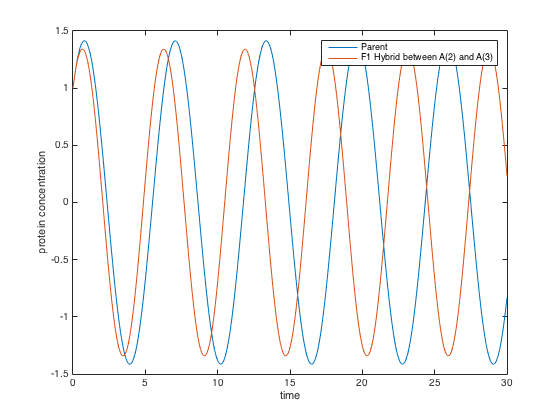
\includegraphics[width=0.5\textwidth]{A2_A3_osci_F1_hyb}
        \end{figure}
      \end{example}

      \begin{example}[F2 Reproductive Incompatibility in an Oscillating Gene Network]
        F2 versus parental expression dynamics. 

        \begin{figure}[H]
          \begin{tabular}{cc}
            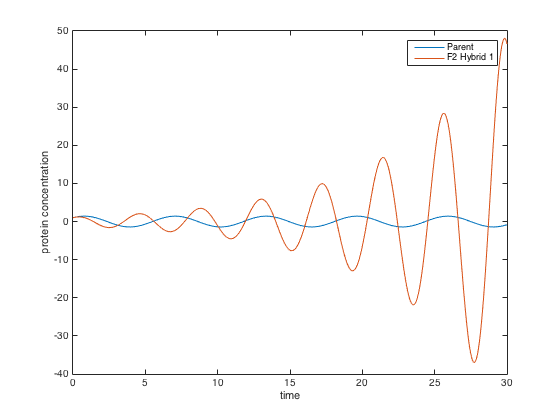
\includegraphics[width=0.2\textwidth]{A2_A3_osci_F2_hyb_1}
            & 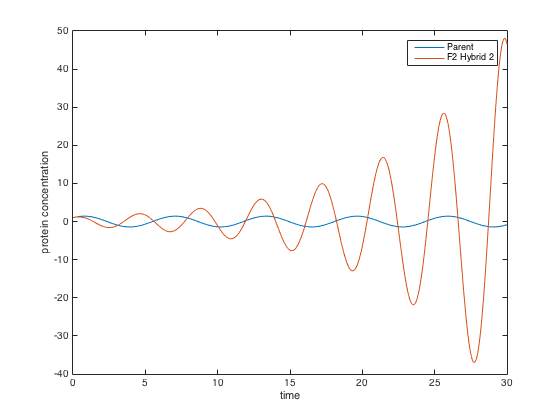
\includegraphics[width=0.2\textwidth]{A2_A3_osci_F2_hyb_2}
           \\ 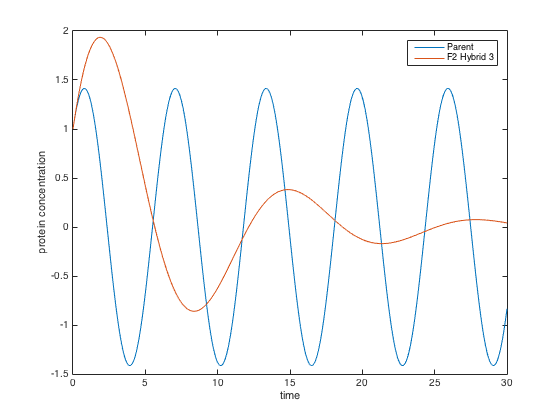
\includegraphics[width=0.2\textwidth]{A2_A3_osci_F2_hyb_3}
            & 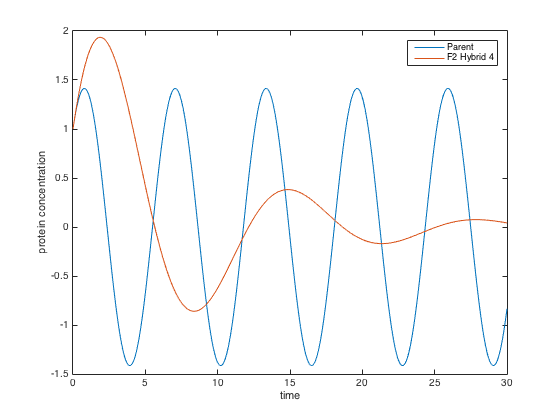
\includegraphics[width=0.2\textwidth]{A2_A3_osci_F2_hyb_4}
            \\ 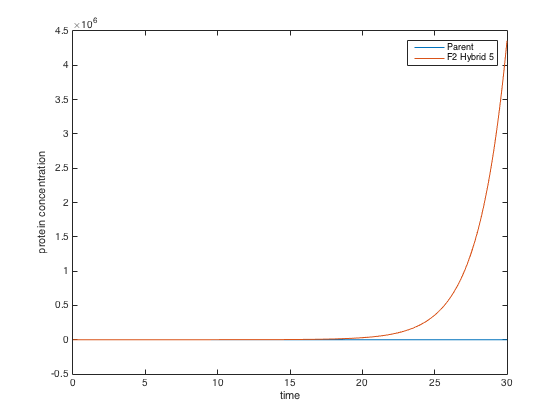
\includegraphics[width=0.2\textwidth]{A2_A3_osci_F2_hyb_5}
            & 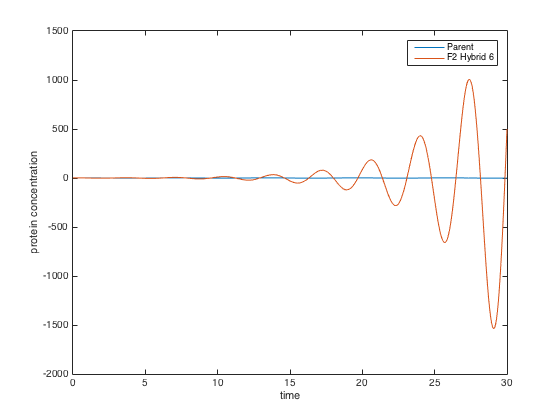
\includegraphics[width=0.2\textwidth]{A2_A3_osci_F2_hyb_6}
          \end{tabular}
        \end{figure}
      \end{example}

      \begin{example}[Not all Networks can Host Incompatibilities]
        convex sets cant have DMIs

        \begin{align*}
          h(t) = 2 e^{- \theta t}
        \end{align*}
        Any non-minimal system with rows summing to $\theta$ is PI. Further, these systems are closed under averaging (mating) and row swapping (meiosis), leaving all hybrids optimally fit. The set of gene matrices is affine and therefore convex.  
      \end{example}

  \section*{Additionl Examples}

    \subsection*{Metabolic Network}

    \subsection*{Gap Gene Network}

    \section*{Discussion}
      \plr{mention $B$ part of genetic architecture}

      \tiny
\bibliographystyle{unsrt}
\bibliography{krefs}
\end{multicols}
\end{document}
